
\documentclass{article}
\usepackage{amsmath,graphicx,mlspconf}

%Select one copyright notice below. Only required for the camera paper submission

%\copyrightnotice{U.S.\ Government work not protected by U.S.\ copyright}
%This will certify that all authors of the Work are U.S. government employees and prepared the Work on a subject within the
%scope of their official duties. As such, the Work is not subject to U.S. copyright protection.

%\copyrightnotice{978-1-4799-1180-6/13/\$31.00 {\copyright}2013 Crown}
%This will certify that all authors of the Work are employees of the British or British Commonwealth Government and
%prepared the Work in connection with their official duties. As such, the Work is subject to Crown Copyright and is
%not assigned to the IEEE. The undersigned acknowledges, however, that the IEEE has the right to publish, distribute
%and reprint the Work in all forms and media

%\copyrightnotice{978-1-4799-1180-6/13/\$31.00 {\copyright}2013 IEEE}
%This is the standard copyright notice which most authors are required to choose

%\toappear{2013 IEEE International Workshop on Machine Learning for Signal Processing, Sept.\ 22--25, 2013, Southapmton, UK}


% Example definitions.
% --------------------
\def\x{{\mathbf x}}
\def\L{{\cal L}}

% Title.
% ------
\title{Cattle Weight Estimation through Image Processing}
%
% Single address.
% ---------------
\name{Sayyada Sahar Fatima, Narjis Zehra, Wahaj Ahmed\thanks{Thanks to Dr. Muhammad Farhan for supporting.}}
\address{}
%
% For example:
% ------------
%\address{School\\
%	Department\\
%	Address}
%
% Two addresses (uncomment and modify for two-address case).
% ----------------------------------------------------------
%\twoauthors
%  {A. Author-one, B. Author-two\sthanks{Thanks to XYZ agency for funding.}}
%	{School A-B\\
%	Department A-B\\
%	Address A-B}
%  {C. Author-three, D. Author-four\sthanks{The fourth author performed the work
%	while at ...}}
%	{School C-D\\
%	Department C-D\\
%	Address C-D}
\usepackage{graphicx} 
\graphicspath{ {images/} }

\begin{document}
%\ninept
%

\maketitle
%
\begin{abstract}
The products in livestock business depends on the weight and body size of the cattle. Weight is the most important factor in Livestock Business. It is very effective in assessing the reproductive efficiency and growth performance of an animal. Weight is also used in measuring the correct dose of therapeutic pharmaceutical to treat animal diseases. The correct amount of feed can also be determined based on the weight to avoid underfeeding or overfeeding [1].

Traditionally there are many ways through which ranchers estimate the weight of cattle. They use a measuring tape to get the measures of different areas of the body and get the weight by applying formulas on these measures. Sometimes they just use their experience and estimate the weight. In large farms the weighing scale is used for the measurement, which is a very tedious task and involves a tremendous amount of manhandling. Also, it takes a lot of time and effort to weigh only a single animal. Since this task is of much importance and has a direct impact on the profit margin of this industry, automation of this task can lead to some significant impact on the profit and can save a lot of effort and time [2]. 
\end{abstract}
%
\begin{keywords}
Livestock, cattle weight, per-pixel depth, heart-girth measurement, digital image processing  
\end{keywords}
%
\section{Introduction}
\label{sec:intro}

In our project, the image processing techniques such as preprocessing, segmentation by using different segmentation method, morphological processing is used to automate the process of weight estimation. Weight is estimated, based on physical characteristics that are visible and measurable. Chest circumference is one of the factor that affects the weight of cattle. It is extracted by applying operations related to image processing. In order to calculate the chest circumference, depth information is also incorporated to extract the per-pixel depth from the camera. 

\section{Literature Review and Hypothesis}
\label{sec:format}
According to the research study, the weight of the cattle can be estimated by calculating the length and chest circumference of the animal. Since, there is a linear relationship between body length, chest circumference and weight of the animal.

According to Sonenarjo (1988) [5], the chest circumference and body weight of cattle there is a positive correlation. This shows that if had known measure of livestock body can then be made an equation that describes the relationship between each the size of linear body with the weight of his body. 

Prandana et al. in [6], captured the front and side images to estimate the weight. The research was done to estimate the cattle’s weight, in which the author detected the largest area using active contour and extracted the number of pixels from the images. In this research, 73\% accuracy was achieved.

Khojastehkey et al. in [7], used the cropped images to get the weight estimate of lambs. The author used the technique of binarization to recognize the images. For this purpose, he separated the background from the foreground. This research results in 89\% of accuracy.

According Soeprapto [4], the body weight of cattle can be calculated by the formula:

\begin{equation}
    BW =\frac{ BL + (CC)^{2}}{10840}
\end{equation}
Where, \textit{BW} is the body weight in kg,
\textit{BL} is the body length in cm,
\textit{CC} is chest circumference in cm.

According to Murtidja [8], the body weight of cattle can be determine using the following formula:

\begin{equation}
    BW = BL * WoC *70
\end{equation}
Where, \textit{BW} is the body weight in kg,
\textit{BL} is the body length in meters (m),
\textit{WoC} is chest circumference in meters (m).

According Schoorl written by Siregar [3], Weight of the cattle can be calculated by only finding the chest circumference of cattle. This relationship between body weight and chest circumference is given as follow.

\begin{equation}
    BW = \frac{ (CC + 22)^{2}}{100}
\end{equation}
Where, \textit{BW }is body weight in kg, and \textit{CC} is chest circumference in cm.


All this research study shows that the weight of the cattle or animal can be obtained from its images by using different techniques in image processing. In the project, only chest circumference/ heart girth measurement is used to calculate the weight of the cattle. 

\section{Methodology}
\label{sec:pagestyle}

In the project, physical characteristic of cattle i.e heart girth length is calculated to determine the weight of cattle. As research study shows that, weight is dependent on physical properties of cattle an can be obtained by finding the physical characteristics that are visible and measurable. 
The following block diagram shows the overall methodology that is used in the project. 
\begin{figure}[h]
    \centering
    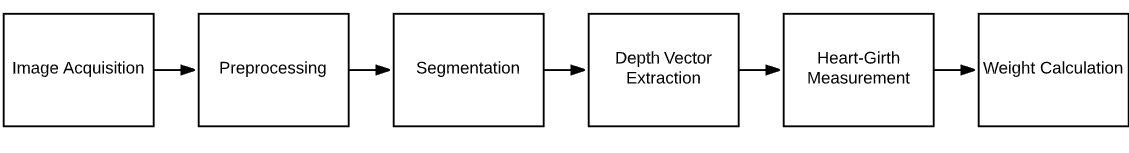
\includegraphics [scale=0.3] {blk}
    \caption{Block diagram of image processing procedures }
    \end{figure}

\subsection{Image Acquisition}

The image of a cattle is captured by a Intel RealSense (D415) depth camera. While capturing the image, the assumption that was taken is that the camera is in a range of 2 to 4 meters away from cattle. Only side view of cattle is captured in order to determine the physical characteristics. 

\subsection{Image Preprocessing}

At this step, all the captured images get preprocessed to apply further image processing techniques. At preprocessing step, some common methods that are also mentioned in research papers are followed. Preprocessing steps that used in the project are as follow.

\begin{enumerate}
    \item Resize the image.
    \item Apply filter to smooth the image and then convert it into YCbCr.
      \begin{figure}[h]
    \centering
    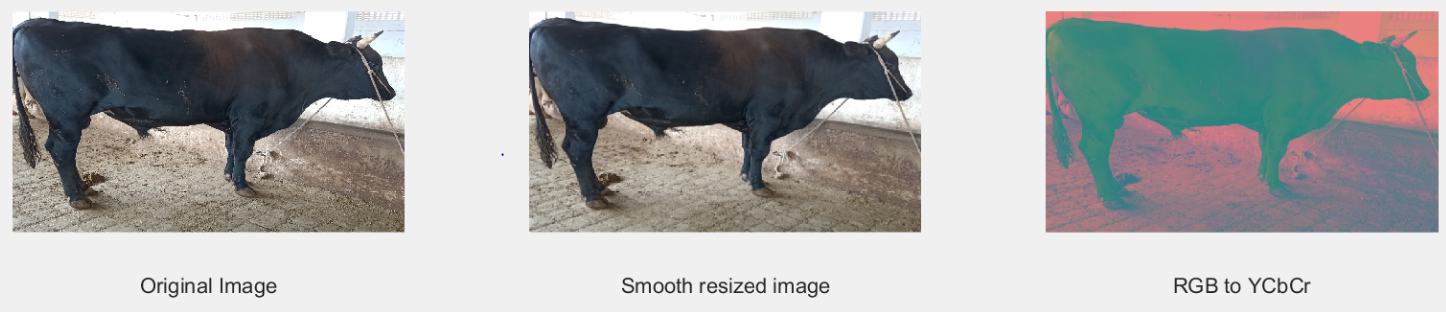
\includegraphics [scale=0.25] {pre}
    \caption{Resizing and Smoothing and conversion into YCbCr }
    \end{figure}
 
    \item Apply different edge detection methods such as sobel, prewitt, and canny to detect the edges and then morphological operations to remove small noisy structures.
    
      \begin{figure}[h]
    \centering
    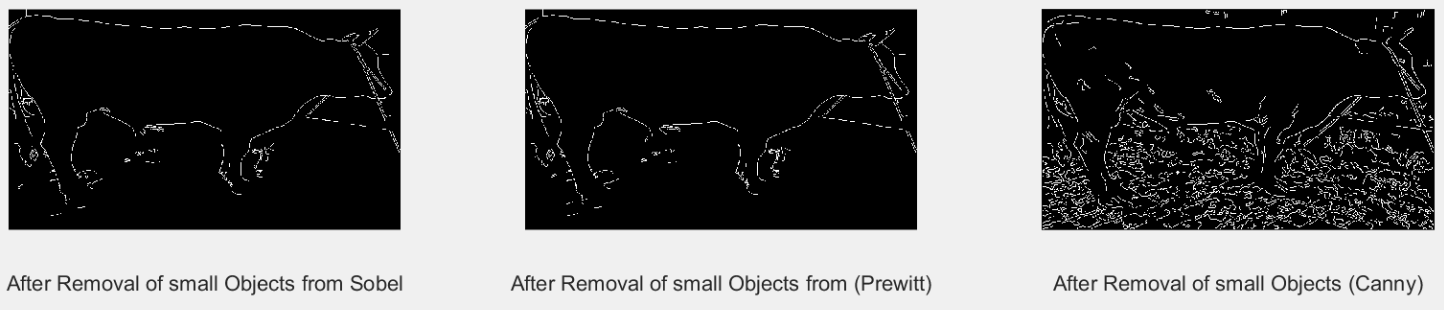
\includegraphics [scale=0.25] {mor}
    \caption{Edge Detection results from Sobel, Prewitt and Canny}
    \end{figure}
    
    \item Apply some morphological operations to make the results, obtained from edge detection step, more better. At this step closing is applied to fill the broken edges.
    
     \begin{figure}[h]
    \centering
    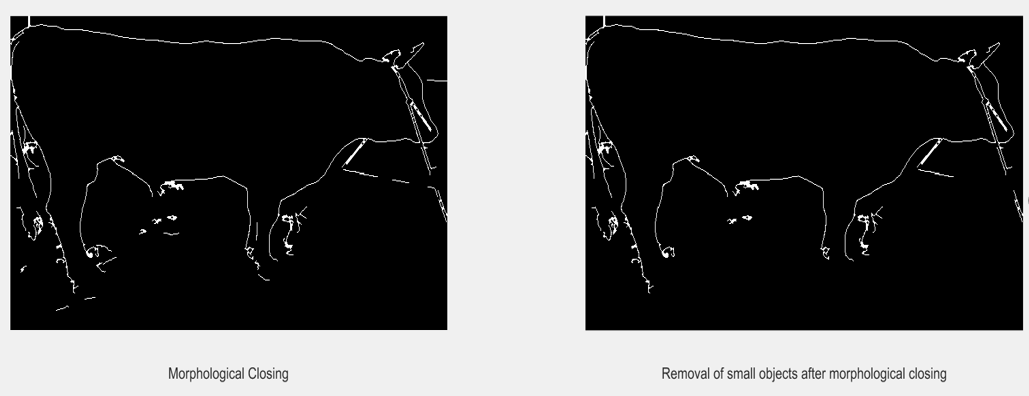
\includegraphics [scale=0.35] {morphological_closing_result}
    \caption{Morphological Processing}
    \end{figure}
    
\end{enumerate}

\subsection{Image Segmentation}

After doing preprocessing on captured image, image segmentation techniques are used to segment out the foreground from background. In the project, different techniques of image segmentation are used on different images depending on the image foreground and background. 
Following are the methods that are used on different images to separate the foreground form background.
\subsubsection{Global Thresholding}
This method works on the principal of global threshold in which a threshold is set for the whole image and the pixel having intensity value equal and above the threshold value is set to foreground pixel otherwise background pixel. When this method is applied on the image in which background and foreground have almost similar intensity values, then this method get failed.

The same method then applied on the image in which the pixel intensity values of two regions i.e foreground and background are very different from each other. It showed a very good results and almost the two regions were segmented out. In order to make the segmentation results more better, morphological operation, erosion is applied to remove the some noisy structures. 

\begin{figure}[h]
    \centering
    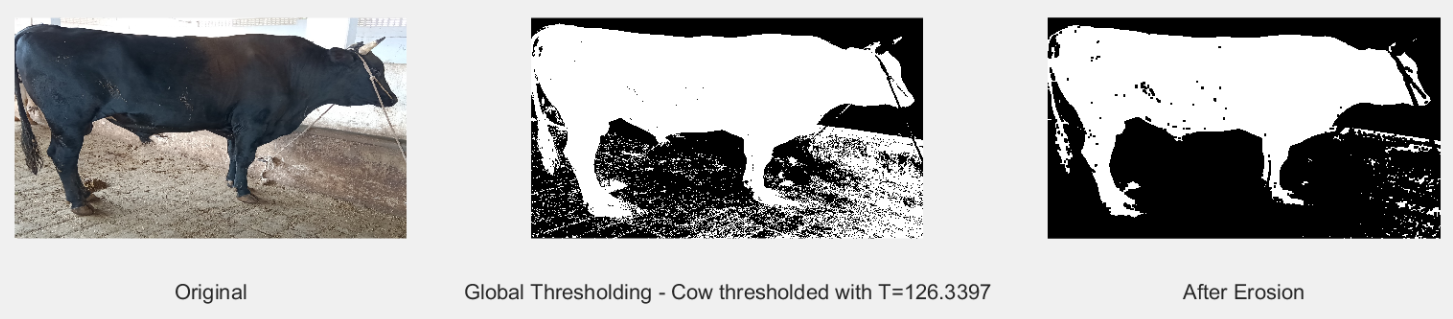
\includegraphics [scale=0.25] {g_t}
    \caption{Global Thresholding followed by Erosion}
    \end{figure}

\subsubsection{Otsu's Thresholding}

This method works similar to the global thresholding method but set multi threshold values (in many case two threshold values) for the image. It works on the principle to maximize the between class variance and minimize the in-class variance.
It provides the best result when histogram of the image is bi-model. Attached below is the result from otsu segmentation which is quite good since the histogram of the original image is almost bi-model. 

\begin{figure}[h]
    \centering
    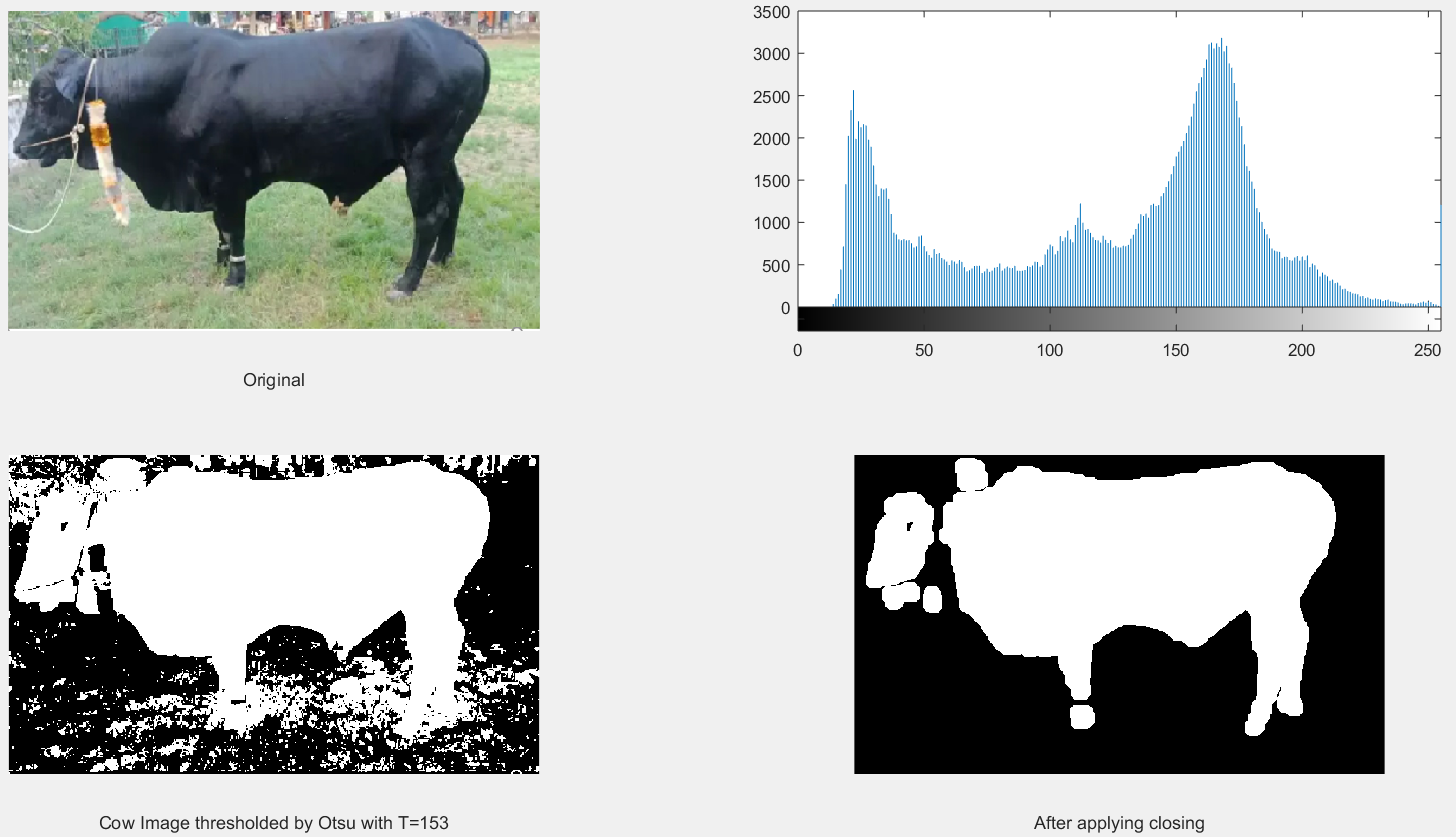
\includegraphics [scale=0.25] {otsu}
    \caption{Otsu's Thresholding}
    \end{figure}

\subsubsection{Region Growing Based Segmentation}

This method segments the region on the bases of intensity. It starts to grow by initializing the seed pixel and then adds the pixel into the region if it has similar intensity as of seed pixel. It gave the best result when cow is of uniform intensity. The result obtained from this method is attached below.

\begin{figure}[h]
    \centering
    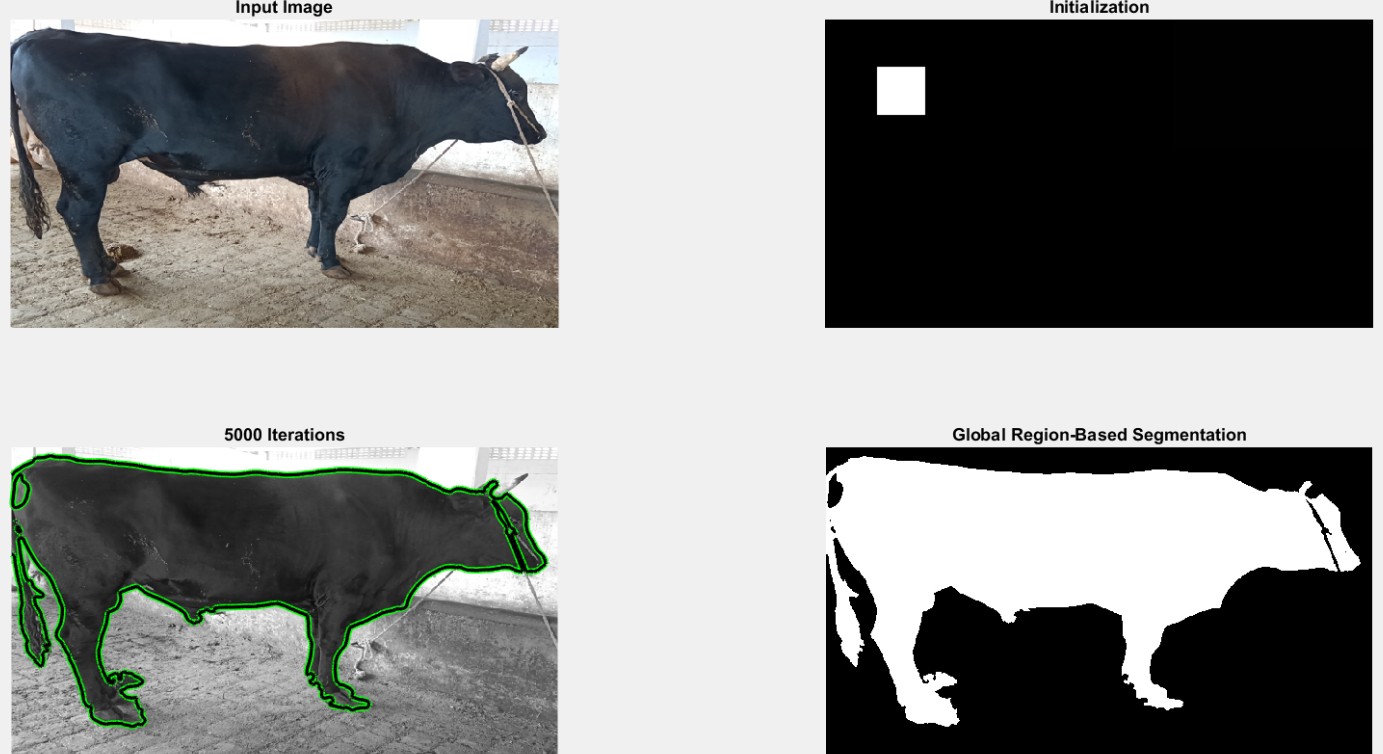
\includegraphics [scale=0.25] {r_g}
    \caption{Region Growing based Segmentation}
    \end{figure}


\subsection{Identifying Heart-Girth Points }

After segmenting the foreground (in our case cow) from background, end points of heart girth are identified. Since the images are captured from depth camera, per pixel depth is known and is saved in a 2D array. Once the points are identified the depth vector is extracted from the 2D array to calculate the arc length. 

\subsection{Heart-Girth Curve Length Estimation}

Once we have a vector of pixels representing the heart girth curve, we can convert it into real world measurements using the procedure defined below. For the simplicity, consider that we have a formula which converts given number of pixels into meters and also take a distance from camera to
take care of the scaling, because otherwise far objects appear small in image. Now
given this formula consider the abdomen of the cattle. It is mostly symmetric from
both sides. If we take the measurements of a heart girth curve on
the surface of the abdomen, which is like a semi-ellipse from one side, will have huge
factor in measurements. So to preserve this information the following procedure is
used.
Now consider the figure below. Here picture of a surface is taken from a dept camera.
Black curve represents the surface and the red lines represent per-pixel distance
from camera. Since, we have a function which can convert number
of pixels covered at certain depth to meters, we can get the measures for each pixel
in meters. But our problem is to get the length of the curve in meters
while preserving the curve, we break the curve into small segments each segment is
break after one pixel. If we have to estimate the curve of this segment we can do so
by fitting a triangle on it and then can use the Pythagoras theorem
to calculate the hypotenuse or the length of the segment since base would be equal to 1 pixel and perpendicular can be determined by taking absolute difference between two consecutive points depth points. We can apply this procedure over all segments and then sum all segments’
length to estimate the length of the curvature. Hence by using this technique we can
get the the length of heart girth circumference more accurately.

\begin{figure}[h]
    \centering
    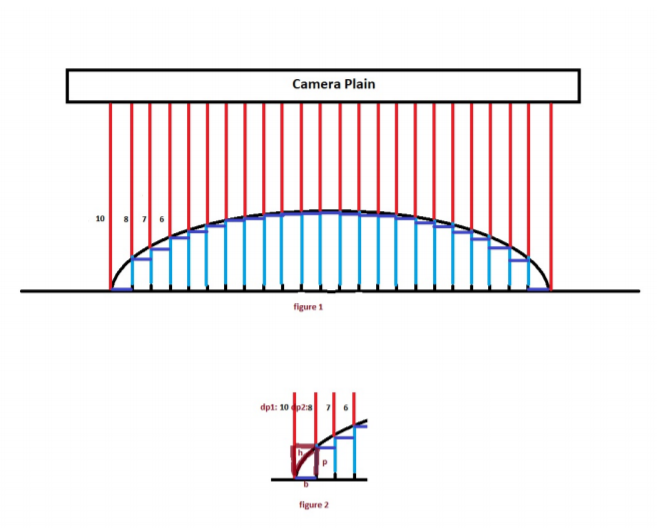
\includegraphics [scale=0.5] {h_g_m}
    \caption{Heart girth measurement technique}
    \end{figure}


\subsection{Calculation Process}
Once we have heart-girth length in meter, it is first converted into centimeters and then can be put in the standardize formula to calculate the weight of cattle.

The formula that is used in the project after getting the length of curve is given as follow.

\begin{equation}
    BW = \frac{ (CC + 22)^{2}}{100}
\end{equation}
Where, \textit{BW }is body weight in kg, and \textit{CC} is chest circumference in cm.
\section{Results and Discussion}
\label{sec:typestyle}

In order to achieve the goal of the project, it means weight estimation of the cattle, the simplest, reliable and more accurate technique is used. The research papers we reviewed did not incorporate the depth information which
in our case would greatly increase accuracy. By incorporating the depth information, we got per pixel depth which we used to determine the curve length. 
Since, we don't have labeled data of the images on which we applied image processing we can not verify our results but on comparing our results with the cow of known weight, we can easily assumed that there would be very least error in our result. 
We tested our methodology on several images and compared our results with the cow of known weight which was 600kg and our results were easily comparable. 
In figure attached below, the left most is the cow with 600kg weight while other two our the cows from our test set 

\begin{figure}[h]
    \centering
    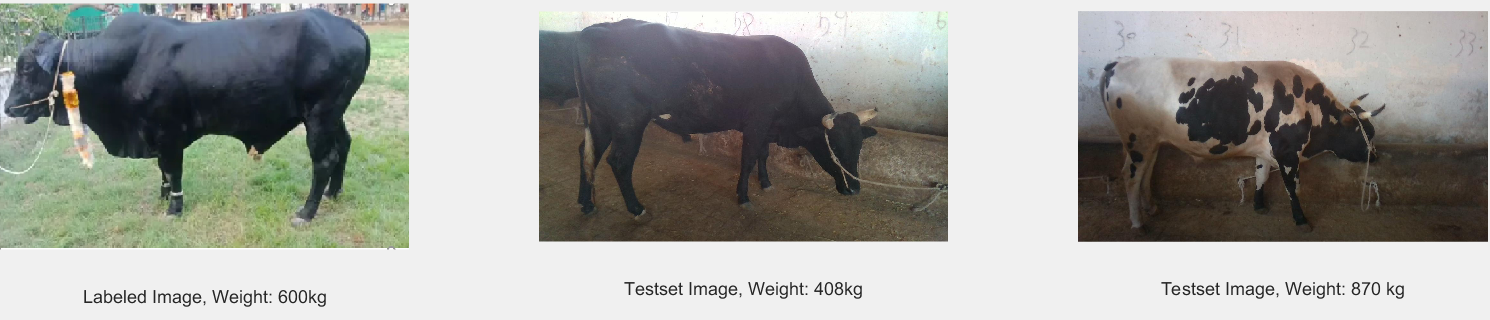
\includegraphics [scale=0.25] {result}
    \caption{Results}
    \end{figure}

\section{Conclusion}
Based on the findings and results obtained after doing the project, it can be concluded that:
\begin{enumerate}
    \item Physical measurements such as heart-girth can be used to obtained the weight of cattle.
    \item Weight of the cattle can be calculated by using image processing techniques.
    \item Depth information or per pixel depth can be used to find the physical measurements more accurately and efficiently.
    \item Once the measurements are known, standardize and globally recognized formulas can be used to determine the weight of cattle. 
\end{enumerate}
\section{Acknowledgement}
The project is done under the supervision of Dr. Muhammad Farhan, Assistant Professor at Habib University, Karachi

\section{REFERENCES}
\label{sec:ref}
\begin{enumerate}
    \item Why Weight and What is EID? (2019). (Datamars Limited) Retrieved from TRU -TEST.
    \item Chintan Bhatt, Aboul-ella Hassanien, "Barqi breed Sheep Weight Estimation based on Neural Network with Regression." (Charotar University of Science and Technology, Gujarat, INDIA
    \item Siregar,S. B.,2007. Fattening Cattle. Jakarta : Penebar Swadaya.
    \item Soeprapto,H., Z.Abidin. 2006. How Fattening Beef Cattle. Jakarta: Agromedia Press
    \item Soenarjo, Ch. 1988. A View Animal Science Lecture. Jakarta: CV. Baru
    \item Pradana Z., B. Hidayat, and S. Darana. 2016. "Beef Cattle Weight Determine by Using Digital Image Processing."
    \item  Mahdi Khojastehkey, Ali Asghar Aslaminejad, Mohammad Mahdi Shariati \& Rouhollah Dianat (2016) Body size estimation of new born lambs using image processing and its effect on the genetic gain of a simulated population, Journal of Applied Animal Research, 44:1, 326-330, DOI: 10.1080/09712119.2015.1031789
    \item Murtidja, B,A. 1993. Breeding Cattle. Yogyakarta : Kanisius
\end{enumerate}





% References should be produced using the bibtex program from suitable
% BiBTeX files (here: strings, refs, manuals). The IEEEbib.bst bibliography
% style file from IEEE produces unsorted bibliography list.
% -------------------------------------------------------------------------
\bibliographystyle{IEEEbib}
\bibliography{strings,refs}

\end{document}
